%% The first command in your LaTeX source must be the \documentclass command.
%%
%% Options:
%% twocolumn : Two column layout.
%% hf: enable header and footer.
\documentclass[
% twocolumn,
% hf,
]{ceurart}

%%
%% One can fix some overfulls
\sloppy

%%
%% Minted listings support 
%% Need pygment <http://pygments.org/> <http://pypi.python.org/pypi/Pygments>
\usepackage{listings}

%% auto break lines
\lstset{breaklines=true}

%%
%% end of the preamble, start of the body of the document source.
\usepackage{float}
\usepackage{url}
\begin{document}

%%
%% Rights management information.
%% CC-BY is default license.
\copyrightyear{2023}
\copyrightclause{Copyright for this paper by its authors.
  Use permitted under Creative Commons License Attribution 4.0
  International (CC BY 4.0).}

%%
%% This command is for the conference information
\conference{Second International Workshop on Linked Data-driven Resilience Research (D2R2'23) co-located with ESWC 2023, May 28th, 2023, Hersonissos, Greece}


%%
%% The "title" command
\title{Truth or Dare: Investigating Claims Truthfulness with ClaimsKG}

%\tnotemark[1]
%\tnotetext[1]{}

%%
%% The "author" command and its associated commands are used to define
%% the authors and their affiliations.

%\cormark[1]
%\fnmark[1]
\address[1]{%Knowledge Technologies for the Social Sciences Department, 
KTS Department, GESIS – Leibniz Institute for the Social Sciences, Cologne, Germany}
\address[2]{Heinrich-Heine-University Dusseldorf, Dusseldorf, Germany}
\address[3]{Institute of Computer Science, FORTH-ICS, Greece}
\address[4]{EuroMov Digital Health in Motion, Univ. Montpellier, IMT Mines Alès, Alès, France}
\address[5]{LIRMM / University of Montpellier / CNRS, France}

\author[1]{Susmita Gangopadhyay}[email=susmita.gangopadhyay@gesis.org,]
\author[1]{Katarina Boland}[email=katarina.boland@gesis.org]
\author[1]{Danilo Dess{\'i}}[email=danilo.dessi@gesis.org,]
\author[1,2]{Stefan Dietze}[email=stefan.dietze@gesis.org]
\author[3]{Pavlos Fafalios}[email=fafalios@ics.forth.gr]
\author[4]{Andon Tchechmedjiev}[email=andon.tchechmedjiev@mines-ales.fr]
\author[5]{Konstantin Todorov}[email=konstantin.todorov@lirmm.fr]
\author[1]{Hajira Jabeen}[email=hajira.jabeen@gesis.org]

%% Footnotes
%\cortext[1]{Corresponding author.}
%\fntext[1]{These authors contributed equally.}

%%
%% The abstract is a short summary of the work to be presented in the
%% article.
\vspace{-4mm}
\begin{abstract}
Searching and exploring online information is fundamental for our society. However, it is common to find inaccurate information on the Internet, that can quickly spread and be hard to identify. Fortunately, today, many fact-checking sources verify online information to provide online users with a means to recognize its truthfulness. These sources use different languages and scoring systems, which makes fact validation challenging and time-consuming. To address this issue, we propose a new release of ClaimsKG, a knowledge graph of about 59,580 claims, which covers  13 different fact-checking sources and provides a structured way to retrieve verified online claims. ClaimsKG is built using a pipeline that makes use of entity linking and disambiguation tools to fetch entities from DBpedia and an ad-hoc scoring normalization system. ClaimsKG is used as a showcase to provide the public with interesting and verified information about events of our times. 
%The wide availability of content on social media has created an environment for 
\end{abstract}
\vspace{-4mm}
%%
%% Keywords. The author(s) should pick words that accurately describe
%% the work being presented. Separate the keywords with commas.
\begin{keywords}
  Claims \sep
  Knowledge Graph \sep
  Fact-Checking \sep
  Entity-Fishing \sep
  RDF
\end{keywords}
\vspace{-4mm}
	
\newcommand{\HJ}[1]{\color{green}}
%%
%% This command processes the author and affiliation and title
%% information and builds the first part of the formatted document.
\maketitle
\vspace{-9mm}
\section{Introduction}
\vspace{-2mm}
Fact-checking is the task of assessing the veracity of claims made by the public. Currently, there is worldwide concern over the spread of fake news and how it affects social, political, and economic well-being. In recent times, we have seen misinformation spreading faster than truth~\cite{vosoughi2018spread}. The dissemination of fake news has sparked widespread interest among researchers and evolved active research directions in the field of automatic fact-checking ~\cite{hassan2015quest}, fake news detection~\cite{tschiatschek2018fake}, or spreading patterns of online discourse~\cite{pennycook2020understanding}. Various fact-checking organizations around the world have employed journalists dedicated to this cause. Large amounts of claims are processed at regular intervals to manually assess their credibility based on sources, facts, and figures. Nevertheless, it is still challenging to grasp the trustworthiness of their content. The reason for this is that fact-checking websites and companies do not express such information in a structured way that might be accessible to the public from a unique entry point and can be processed by machines to provide a variety of services. For example, among the existing fact-checking sources,  \textit{Politifact} uses ``correct", \textit{Snopes}  uses ``Correctly Attributed", while \textit{AFP Factuel} uses ``Vrai"  to state that a claim reports a truth. This makes the task of interpreting and understanding Internet content difficult.  Thus, novel ways to access and use online information are demanded. To fulfill this need,  ClaimsKG, an RDF knowledge graph (KG) of fact-checked claims, enabling structured queries about their truth values, authors, dates, related entities, and metadata, was released in 2019~\cite{tchechmedjiev2019claimskg}.  ClaimsKG makes it easier for users to explore claims in a standardized manner, enabling the discovery and search of fact-checked online information. However, as a result of the dynamic nature of Internet content and fact-checking source websites,
 ClaimsKG is continuously evolving. This paper presents the latest release of ClaimsKG named \textit{ClaimsKG (Aug2022)} which is generated by a pipeline that periodically harvests data from popular fact-checking sources.  Furthermore, claims and their review articles are enriched with entities from DBpedia using a state-of-the-art entity-linking tool. The collected information is described using a specifically designed RDFS model based on well-established vocabularies such as 
\textit{Schema.org}\footnote{Schema.org: \url{https://schema.org}} and \textit{NIF}\footnote{NIF: \url{https://persistence.uni-leipzig.org/nlp2rdf/}}.  Lastly, to simplify the comprehension of claim veracity for users, we introduced a 
\textit{Normalized Truth Rating}\footnote{Normalized Truth Rating: \url{https://data.gesis.org/claimskg/ratings.pdf}} scheme, containing four generic categories: \textit{TRUE, FALSE, MIXTURE,} and \textit{OTHER}. ClaimsKG will be released at regular intervals, maintaining the pipeline updated with state-of-the-art tools and methods, and covering a larger set of fact-checking sources.  
The contribution of this paper is threefold: \vspace{-2mm} 
\begin{itemize}
  \item We present the latest release of ClaimsKG, the largest collection of multilingual claims and associated metadata.
  
  \item We describe the novelties of the ClaimsKG construction process, resulting data and release its source code\footnote{Extractor source code: \url{https://github.com/claimskg/claimskg-extractor/tree/latest\_release}}\textsuperscript{,}\footnote{Generator source code: \url{https://github.com/claimskg/claimskg\_generator/tree/latest\_release}}.
  
  \item We present various use cases using federated SPARQL queries to uncover information that would be difficult or impossible to discover without ClaimsKG. 
 
 % \item The latest release is also multilingual and has claims in other languages apart from English to support a wider group of researchers. %to demonstrate advanced information discovery and exploitation of data.
\end{itemize}
\vspace{-7mm}
\section{Related work}
\vspace{-2mm}

Several studies have utilized machine learning to identify fake news, and one such approach is the Deep Triple Network (DTN)~\cite{LIU2021100646} that employs knowledge graphs to aid in detecting fake news, along with triple-enhanced explanations. The DTN utilizes background knowledge graphs, including open knowledge graphs and graphs extracted from news databases, for feature extraction to classify the news article. The work in~\cite{inbook} semantically detects fake news that utilizes relational features, such as sentiment, entities, and facts directly extracted from the text. They demonstrate that the inclusion of semantic features leads to improved accuracy in classifying fake news. Sciclops~\cite{smeros2021sciclops} proposes a method involving extraction, clustering, and contextualization for analyzing scientific claims in social media posts. A recent survey~\cite{opdahl2022semantic} has examined the utilization of semantic KGs in the integration of heterogeneous news information. While it shows that there has been previous work on data provision for claims detection, e.g., the work in~\cite{shaar-etal-2020-known} which provides a static data set for claims detection, no other dataset is mentioned that could be compared to ClaimsKG, which is a verified claim collection of continuous longitudinal nature  (i.e., a systematic, ongoing process of claims collection).

\begin{table}[t]
\scriptsize
\centering
\caption{Statistics about claims harvested from each website (as of Aug 2022)}\label{statistics-table}
\begin{tabular}{|l|c|c|c|c|c|c|c|c|}
\hline
\textbf{Websites} &  
\textbf{URL} &
\textbf{\begin{tabular}[c]{@{}l@{}}Total\\ Claims\end{tabular}} & 
\textbf{\begin{tabular}[c]{@{}l@{}}Total \\ Entities\end{tabular}} & 
\textbf{\begin{tabular}[c]{@{}l@{}}True \\ Claims\end{tabular}} &
\textbf{\begin{tabular}[c]{@{}l@{}}False \\ Claims\end{tabular}} &
\textbf{\begin{tabular}[c]{@{}l@{}}Mixture \\ Claims\end{tabular}} & 
\textbf{\begin{tabular}[c]{@{}l@{}}Other \\ Claims\end{tabular}} \\ \hline
 
\textbf{Global}  & NA       & 59,580        & 1,371,271         & 7,151        & 30,858        & 10,790          & 10,781        \\ \hline
\textbf{Politifact }  &{\url{https://politifact.com}}    & 21,450        & 354,653          & 2,501        & 8,353         & 6,733           & 3,863         \\ \hline
\textbf{Snopes}  & {\url{https://snopes.com}}       & 14,031        & 481,199          & 2,843        & 6,803         & 2,556           & 1,829         \\ \hline
\textbf{AFP Factcheck} & {\url{https://factcheck.afp.com}}  & 5,058         & 151,208          & 3           & 4,147         & 97             & 811          \\ \hline
\textbf{AFP Factuel(FR)} &{\url{https://factuel.afp.com}}  & 935          & 18,739           & 5           & 627          & 94             & 209          \\ \hline
\textbf{Checkyourfact} & {\url{https://checkyourfact.com}}  & 3,971         & 16,699           & 233         & 3,691         & 4              & 43           \\ \hline
\textbf{Vishva news} &{\url{https://www.vishvasnews.com}}     & 3,490         & 8,930            & 0           & 2,933         & 565            & 0            \\ \hline
\textbf{Fullfact}  &{\url{https://fullfact.org} }      & 2,928         & 6,870            & 403         & 729          & 152            & 1,644         \\ \hline
\textbf{Truth or Fiction} &{\url{https://truthorfiction.com}} & 2,908         & 21,298           & 853         & 260          & 14             & 1,781         \\ \hline
\textbf{Africacheck}  &{\url{https://africacheck.org}}    & 2,854         & 11,448           & 197         & 2,364         & 258            & 35           \\ \hline
\textbf{Fatabyyano} &{\url{https://fatabyanno.net}}      & 1,379         & 101             & 46          & 820          & 4              & 509          \\ \hline
\textbf{Factograph} &{\url{https://factograph.info} }   & 255          & 1,201            & 19          & 69           & 144            & 23           \\ \hline
\textbf{Eu Factcheck} &{\url{https://eufactcheck.eu}}   & 297          & 5,699            & 48          & 48           & 159            & 42           \\ \hline
\textbf{Polygraph}  &{\url{https://polygraph.info}}    & 24           & 293,226          & 0           & 14           & 10             & 0            \\ \hline
\end{tabular}
\vspace{-4mm}
\end{table}

\vspace{-3mm}
\section{ClaimsKG (Aug/2022) Overview and Statistics}
 \vspace{-2mm}
This section describes the latest release of ClaimsKG (available at \url{https://doi.org/10.7802/2469}) and reports its statistics.
 ClaimsKG contains $59,580$ claims harvested from $13$ popular fact-checking sources. The websites are selected based on the International Fact-Checking Network’s (IFCN)\footnote{\url{https://www.poynter.org/ifcn/}} signatories list and considered only sources
referred by the fact-checking community as highly reputable. The list of covered sources is mentioned in Table~\ref{statistics-table}. 
As part of the new release, we have crawled new claims from the fact-checking sites that were included in the previous release and added \textit{Factograph}, \textit{Fatabyanno}, \textit{Eufactcheck}, \textit{Vishvasnews} and  \textit{Polygraph}. This release does not contain  claims from  \textit{Factscan.ca} since its website is no longer online. However, past harvested data from \textit{Factscan.ca} will still be available in previous ClaimsKG releases. Harvested sources contain claims in various languages like English, French, Russian, Urdu, Hindi, Punjabi, Assamese, Tamil, Malayalam, Gujarati, Telegu, Marathi, Odia, and Bengali, thus making it interesting for a broad audience. The time frame for collected claims ranges from 1996 to August 2022. Since these sources were launched at different points in time, the start year for the earliest claims of each website is different. This allows the study of a multitude of entities through fact-checked claims that are contained by the sources and provides the users with the possibility to study events over a long period. In the latest version, the earliest claim from the year 1996  belongs to the website Snopes. This claim describes ``A hostess named Deborah Gail Stone working the America Sings attraction was crushed to death by a rotating wall.", labeled as ``True". Towards the end of the pipeline (see Section~\ref{pipeline}) and after each run we generate statistics, both global and per source, to monitor the health of the extracted data and also to keep track of the recent changes in the websites. Table~\ref{statistics-table} provides information on the total number of claims collected from each of these sources, the total number of entities mentioned in these claims and their reviews, and the veracity label of claims obtained from each website. %The detailed statistics present on the website provide thorough 
 One can find further information such as the percentage of claims that contain date published and author names, the number of entities per review, the number of entities per claim, and the total number of keywords for each fact-checking source on ClaimsKG website (see Table \ref{data-table}).  For other information such as the latest data dump, SPARQL query endpoint, usage instructions, and source code, refer to Table \ref{data-table}. The latest release of ClaimsKG supersedes the previous versions as it contains all the claims from the previous
versions together with additional claims as well as improved entity annotations.
\vspace{-2mm}


\section{ClaimsKG Pipeline}\label{pipeline}
\vspace{-2mm}
In this section, we discuss the processing pipeline of ClaimsKG and also discuss the updates for the newest release. %changes and improvements carried out in the 
%updates for the current release. %It 
The pipeline consists of two major building blocks, namely the Extractor and Generator. %Hereafter, we explain 
The steps of the pipeline are summarized in Figure~\ref{fig1}. 
\vspace{-2mm}
\begin{figure}[ht]
\centering
\caption{Pipeline of ClaimsKG depicting all its modules}
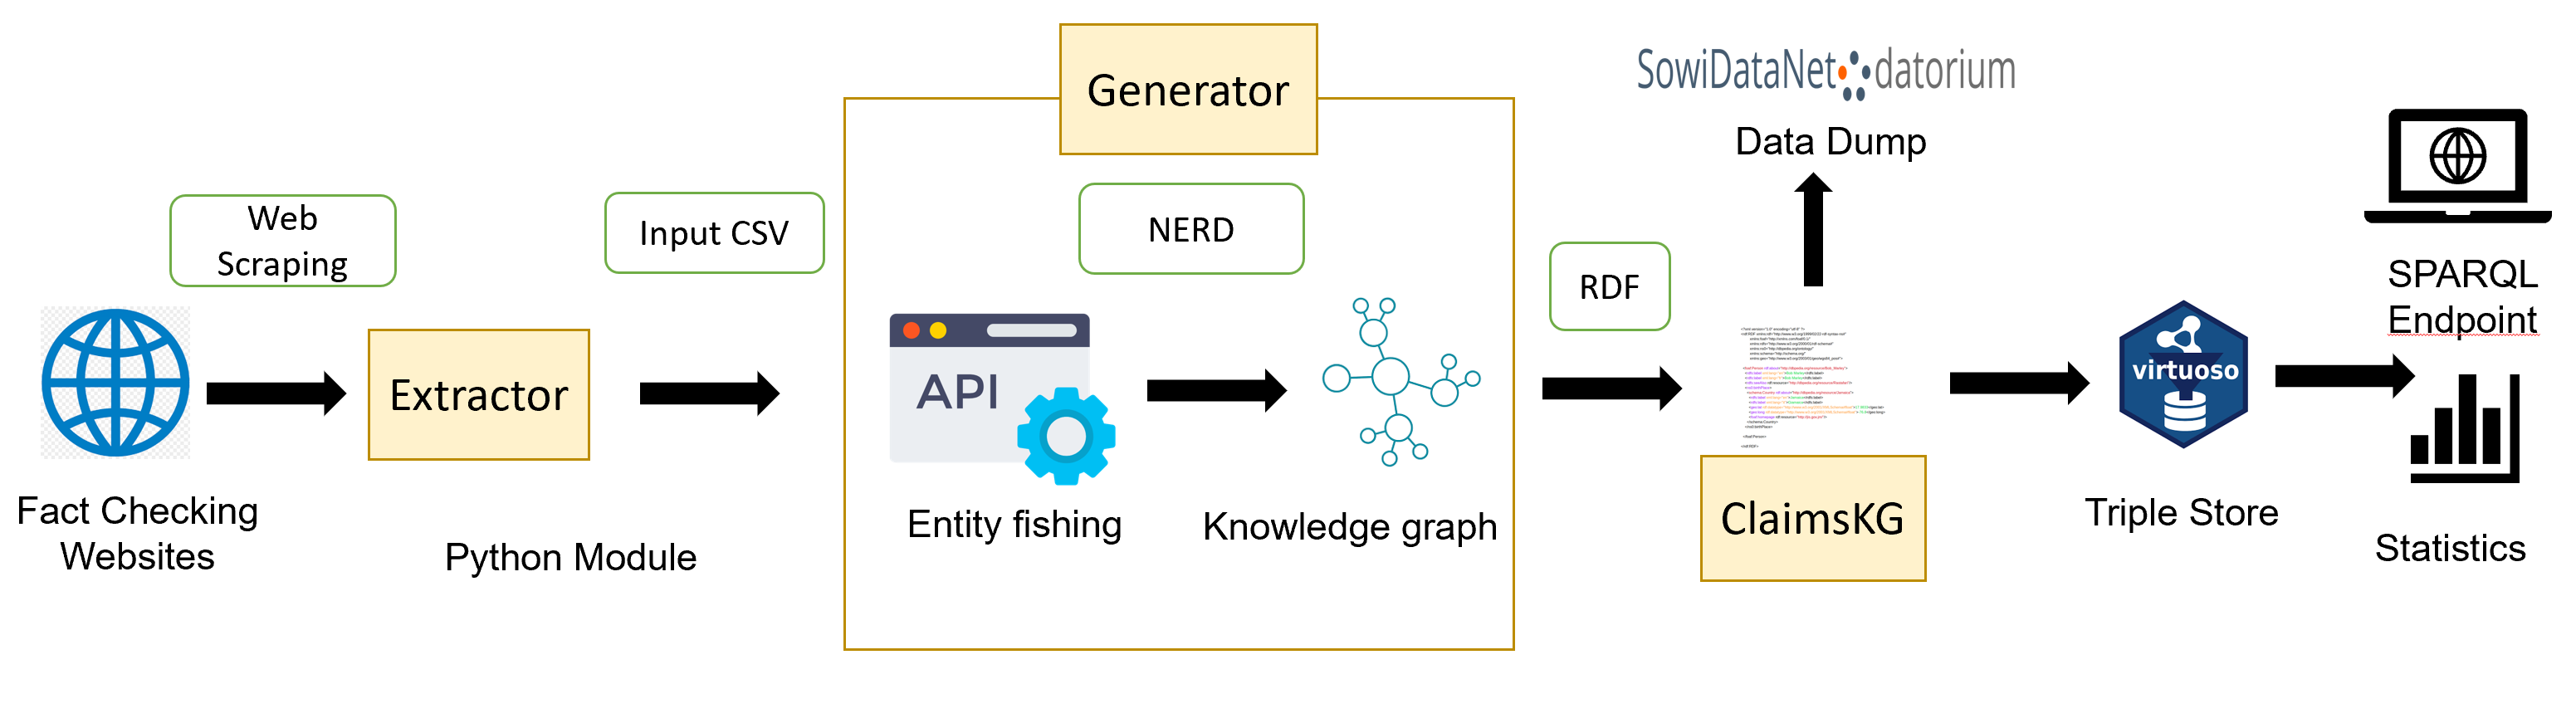
\includegraphics[width=0.75\linewidth]{claimkg}
\vspace{-8mm}
\label{fig1}
\end{figure}

\begin{table}[t]
\scriptsize
\centering
\caption{Links to ClaimsKG data and tools}
\label{data-table}
\begin{tabular}{|l|l|}
\hline
\textbf{Data/Tools} & \textbf{Links} \\ \hline
ClaimsKG Website & \url{https://data.gesis.org/claimskg/}        \\ \hline
Dataset Download                       & \url{https://doi.org/10.7802/2469}                  \\ \hline
Previous Versions                      & \url{https://zenodo.org/record/3518960}             \\ \hline
DCAT Description                       & Included in the KG                            \\ \hline
SPARQL Endpoint                        & \url{https://data.gesis.org/claimskg/sparql}        \\ \hline
Claims Ontology                        & \url{https://data.gesis.org/claimskg/\#Data-model}  \\ \hline
Source Code                            & \begin{tabular}[c]{@{}l@{}}\url{https://github.com/claimskg/claimskg-extractor/tree/latest\_release}\\ \url{https://github.com/claimskg/claimskg\_generator/tree/latest\_release}\end{tabular}                 \\ \hline
ClaimsKG Explorer   \cite{gasquet2019exploring}                   & \url{https://data.gesis.org/claimskg/explorer} \\ \hline
\end{tabular}
\vspace{-4mm}
\end{table}
\vspace{-4mm}

\subsection{\textbf{Extractor}}
In the Extractor module, we perform web scraping of the identified sources. The web-crawling process is different for each source since it is tailor-made and adapted to the structure of each website. For this release, we added five new sources which needed new ad-hoc sub-modules. This module collects the information in a JSON  and consolidates it as a CSV file. The data consists of the claim text, its truth value or original rating, the claim body, a link to the claim review from the fact-checking website, the references cited in the claim reviews, the author of the claim, the author of the review, the date of publication
of the claim, the date of the review if available, the title of the review article, and a set of topic keywords extracted from the source websites if available. This module's main pipeline and working mechanism to harvest data have remained similar to the previous ClaimsKG-generating pipeline but we have made changes according to newly added sources. This module does not perform any data processing so that the time for harvesting the source websites is not overloaded with additional computation.
%keywords extracted from the websites acting as topics.

\vspace{-4mm}
\subsection{\textbf{Generator}} The output of the Extractor serves as input to the Generator. The Generator performs: i) entity annotation and linking ii) rating normalization, and iii) lifting and serialization.

\vspace{-4mm}
\subsubsection{\textbf{Entity Annotation and Linking}}
\vspace{-1mm}
In this phase, we perform Named Entity Recognition and Disambiguation (NERD) of the claims and their reviews. %Currently, the annotation task is performed in the Generator as opposed to the Extractor, which was done in the previous releases.
Differently from the previous pipeline, the entity annotation task is performed within the \textit{Generator} so that it can be applied to the whole downloaded corpus of fact-checked claims at once. This allows a better separation of various modules of the pipeline, making it easy to maintain. %We perform the annotation task in the Generator to make our pipeline faster in retrieving from the web by separating the data collection from the data processing steps. 
One major update in this module is the use of Python Entity Fishing Client (PEFC)\footnote{\url{https://github.com/kermitt2/entity-fishing}} instead of TagMe\footnote{\url{https://sobigdata.d4science.org/web/tagme/tagme-help}}. 
The reason for this choice is twofold: (i) TagMe code is legacy and we wanted to move to a more recent and easily deployable service, (ii) PEFC supports multilingual claims in ClaimsKG and performs entity recognition and disambiguation against Wikidata in 11 different languages (English, French, German, Italian, Spanish, Arabic, Mandarin, Russian, Japanese, Portuguese, and Farsi).
PERC uses GROBID-NER\footnote{\url{https://github.com/kermitt2/grobid-ner}}, a Named-Entity Recogniser based on GROBID for recognizing the Entities. GROBID-NER has 27 Named Entity classes and is specifically dedicated to supporting the resolution and disambiguation of entities against Knowledge Bases. We use SPARQL queries through the Entity Fishing API to fetch DBpedia entities. We run a local version of the NERDClient, using the latest available dump of Wikipedia and Wikidata on Feb 1, 2022, as reported in the guideline\footnote{\url{https://nerd.readthedocs.io/en/latest/build.html}}. 
\vspace{-4mm}

\subsubsection{\textbf{Rating Normalization}} 
\vspace{-1mm}
We observed that fact-checking source websites have different rating systems with non-uniform labels. For example, Politifact uses labels like ``Pants on Fire"  while AFP Factcheck has values like ``Misleading", and ``Satire". To make the rating uniform, we provide a normalized rating score for all claims in the dataset, alongside the original ratings. We classified sources into four categories \textit{TRUE, FALSE, MIXTURE, OTHER} respectively indicated  within ClaimsKG with rating values 3, 1, 2, -1, and only labeled a claim as \textit{TRUE} or \textit{FALSE} if it was completely true or completely false and did not have any ambiguity in their ratings. \textit{MIXTURE} is assigned to claims which hold a degree of both truth and falsehood, such as ``half-true", ``Truth! But Postponed!", or ``misleading". \textit{OTHER} is for claims that do not fit into the TRUE/FALSE or MIXTURE categories and has rating names like ``Pending Investigation" or ``photo out of context", among several others. The entire approach to rating normalization is similar to what was performed in the previous releases. In the newest version of the generating pipeline, this module has been extended to normalize the ratings of the newly added sources. % In this release, we added more ratings from the newly added websites to make it more comprehensive.

\begin{figure}[ht]
\centering
\caption{Sample output of a claim from the website TruthorFiction.}
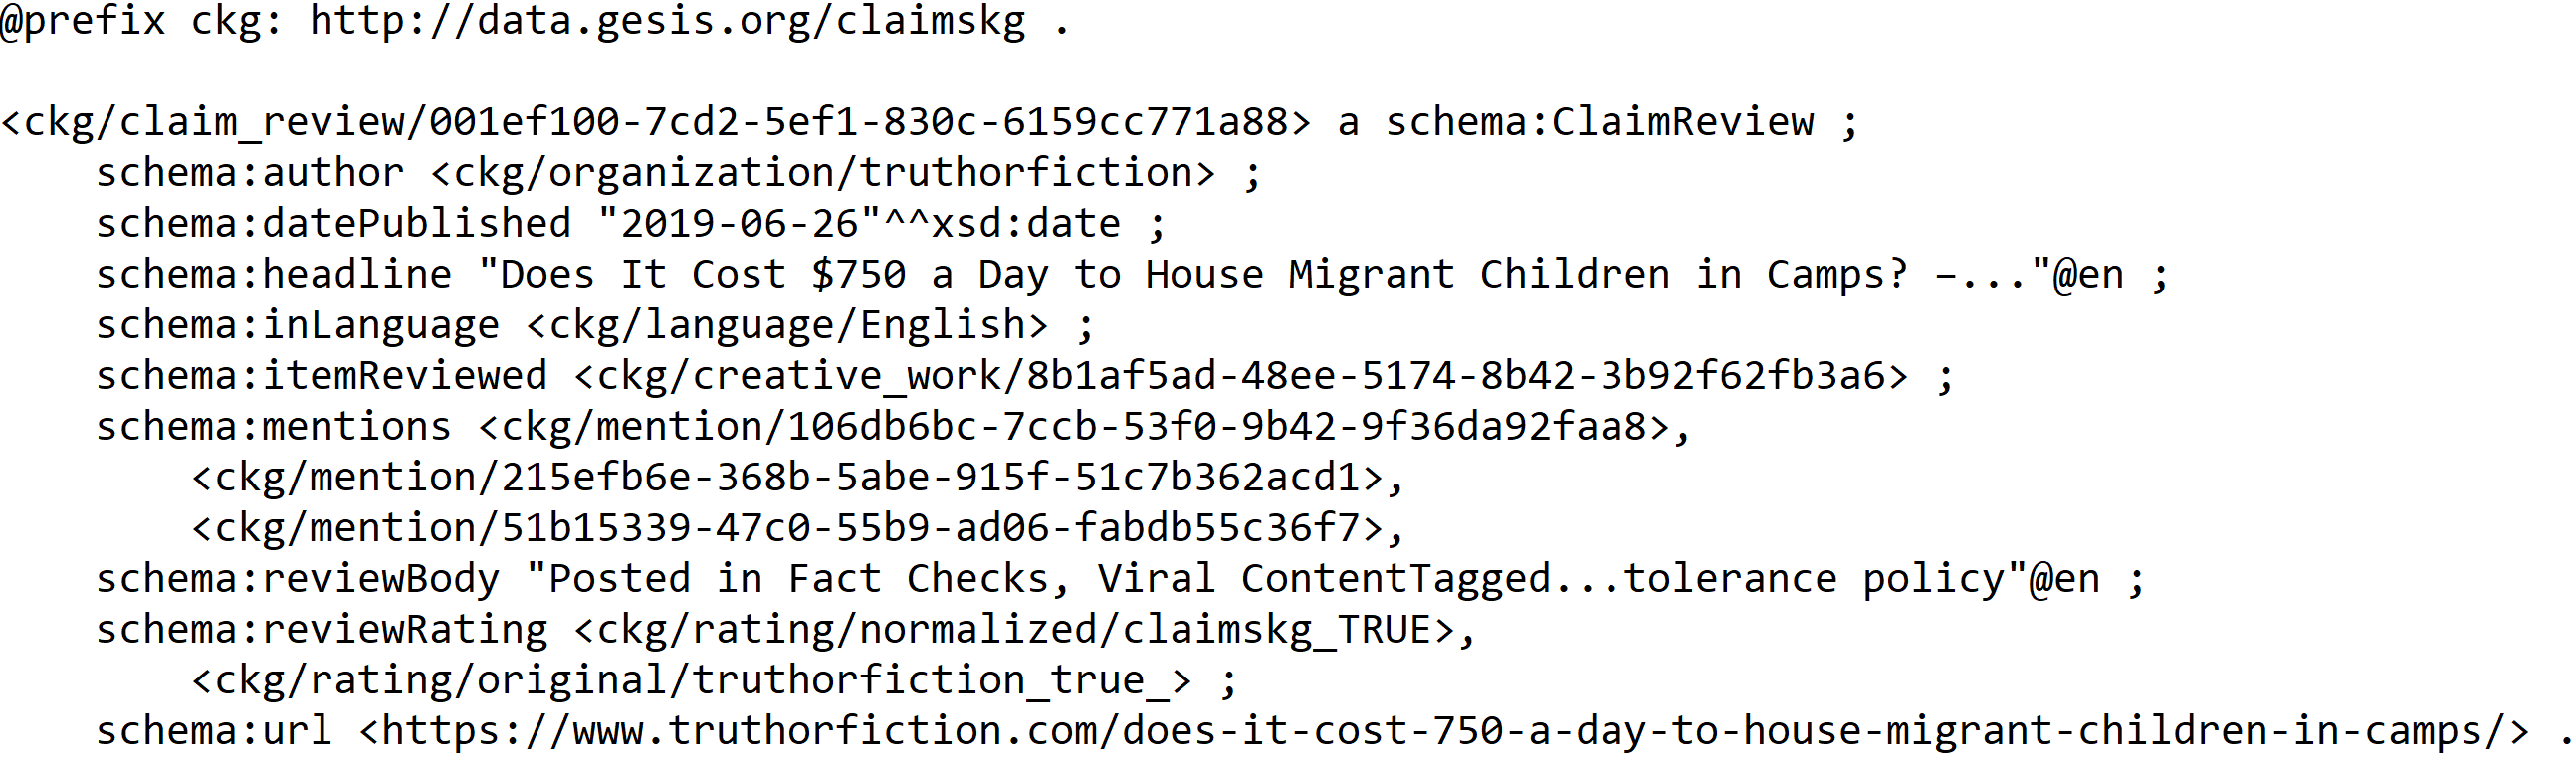
\includegraphics[width=0.75\linewidth]{output.PNG}
\vspace{-4mm}
\label{output_figure}
\end{figure}

\vspace{-2mm}
\subsubsection{\textbf{Lifting and Serialization}} 
The data model of the KG is available on the ClaimsKG website mentioned in Table \ref{data-table}.  We used the \textit{Rdflib}\footnote{Rdflib: \url{https://rdflib.readthedocs.io/en/stable/}} python library to create the model and an abstract RDF graph to then serialize it in
one of the supported formats\textit{ (TTL,n3, XML,nt, pretty-xml,trix, trig, and nquads)}. We generate unique URI identifiers as UUIDs that are
based on a one-way hash of key attributes for each instance. We present an exemplary claim in Figure \ref{output_figure}. %The reader can find technical details and usage instructions following the URLs in Table~\ref{data-table}.
\vspace{-4mm}

\section{Use-cases}
\vspace{-2mm}
The publication of the latest release of ClaimsKG facilitates the uncovering of several %implicit and explicit 
relations, patterns, and trends between the entities, claims, and their sources. The  \textit{SPARQL query endpoint}\footnote{SPARQL query endpoint: \url{https://data.gesis.org/claimskg/sparql}} allows the fetching of information about specific entities and also supports the execution of federated queries from external knowledge bases like DBpedia. Here we present a few of the use cases as an example of what could be achieved using ClaimsKG. 
\vspace{-4mm}
\subsection{ClaimsKG and Corona Virus}
\vspace{-2mm}
The query in Figure~\ref{fig:corona}(a) finds all claims mentioning \textit{Coronavirus}. For each claim, it returns the text, the date, the rating, and the review URL by the fact-checking website. We can further drill down to finding only false claims about Coronavirus for a particular year by adding the ``ratingValue=1" filter, as mentioned in Figure~\ref{fig:corona}(b). This query returns, among many claims, the following one ``Eating bananas is a preventative against the COVID-19 coronavirus disease." along with its date published \textit{(2020-03-22)} and link to the original fact check webpage \url{https://www.snopes.com/fact-check/bananas-coronavirus/}. The result of this query shows how ClaimsKG can bring claims from different fact-checking sources about one topic in one place, which makes it easier and time-saving for the exploration of facts for a user. Searching for the same result manually would have been extremely laborious or unfeasible. A user would have to visit each website and search for claims related to a particular entity or topic (in this case \textit{Coronavirus}), which might or might not be allowed for the source website, and would have to manually look for the claims belonging to a particular veracity label.

\vspace{-1mm}
\begin{figure}\begin{tabular}{cc}
     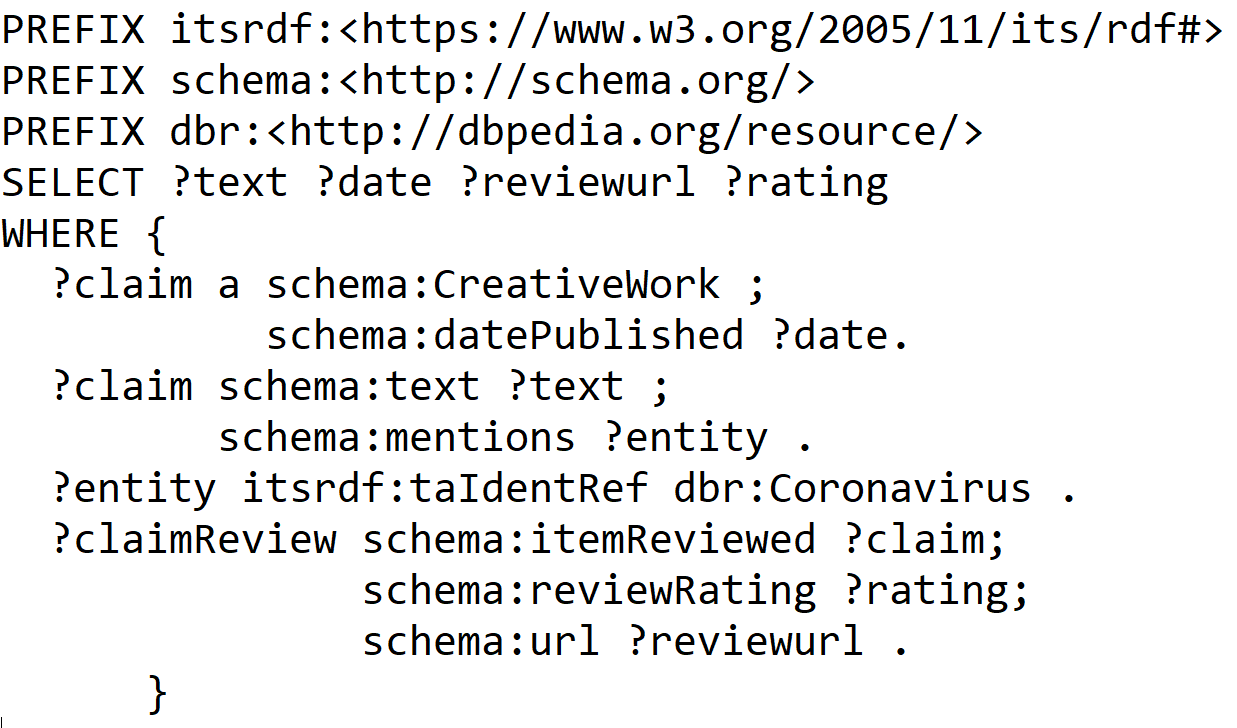
\includegraphics[width=0.40\linewidth]{Table3.PNG}& 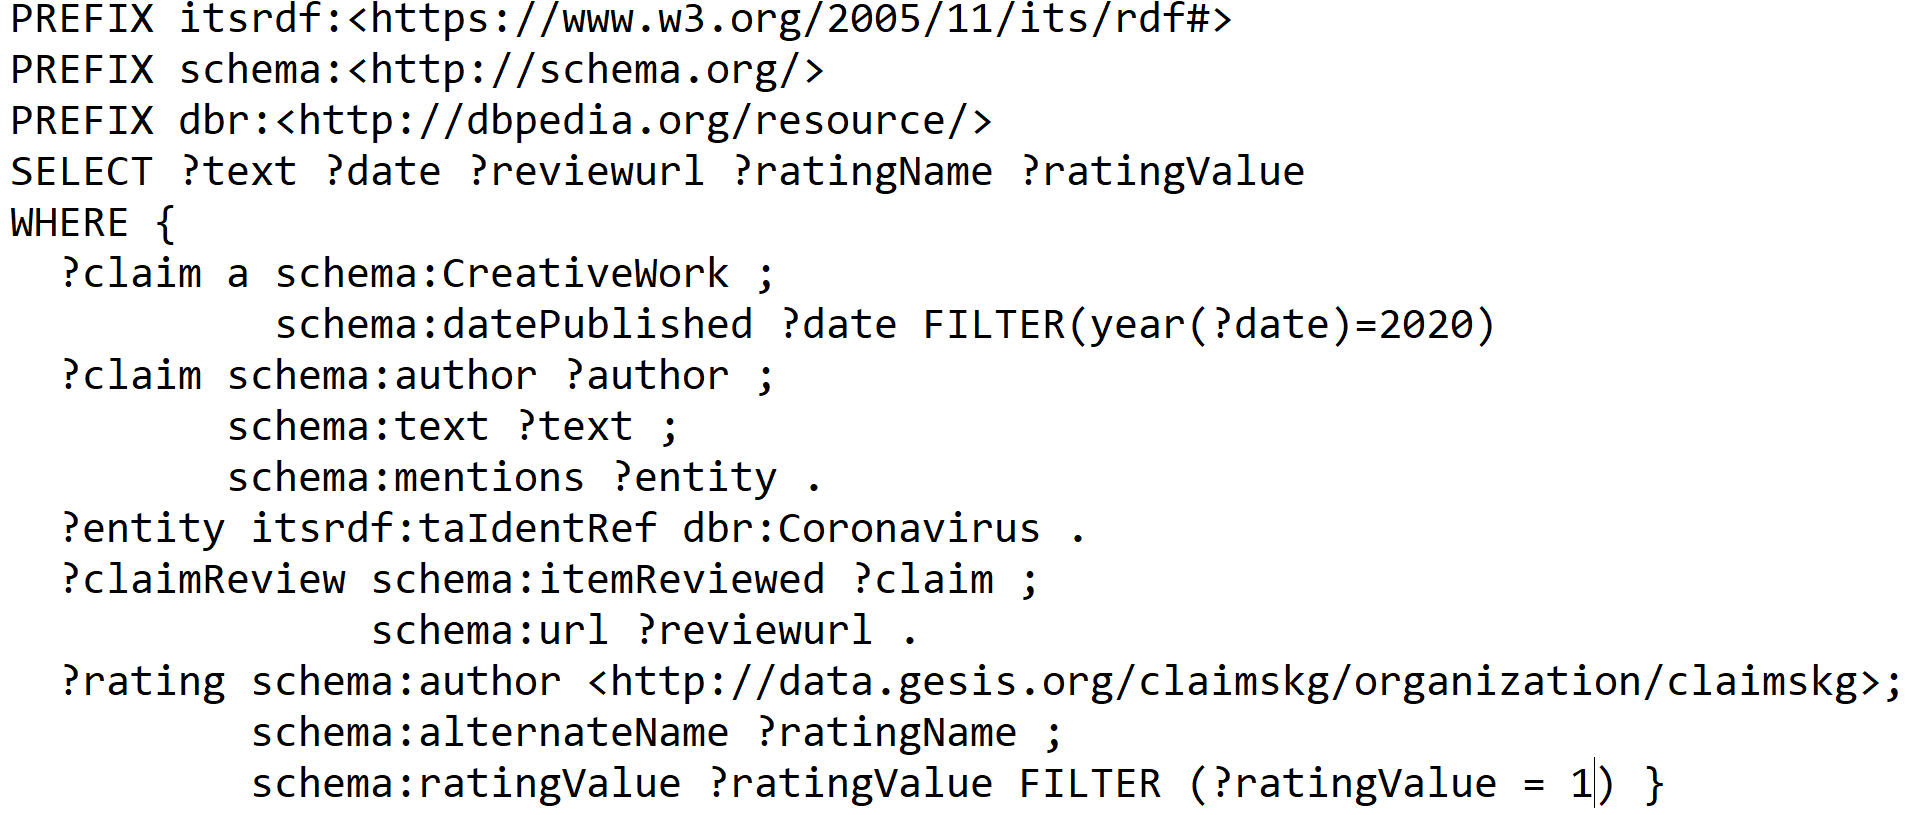
\includegraphics[width=0.55\linewidth]{test1.PNG} \\
     (a) & (b)  
\end{tabular}
    \caption{(a) SPARQL query to fetch all claims related to Coronavirus. (b) SPARQL query to fetch all false claims relating to Coronavirus for the year 2020.}
    \vspace{-4mm}
    \label{fig:corona}
\end{figure}

\begin{figure}
    \begin{tabular}{cc}
    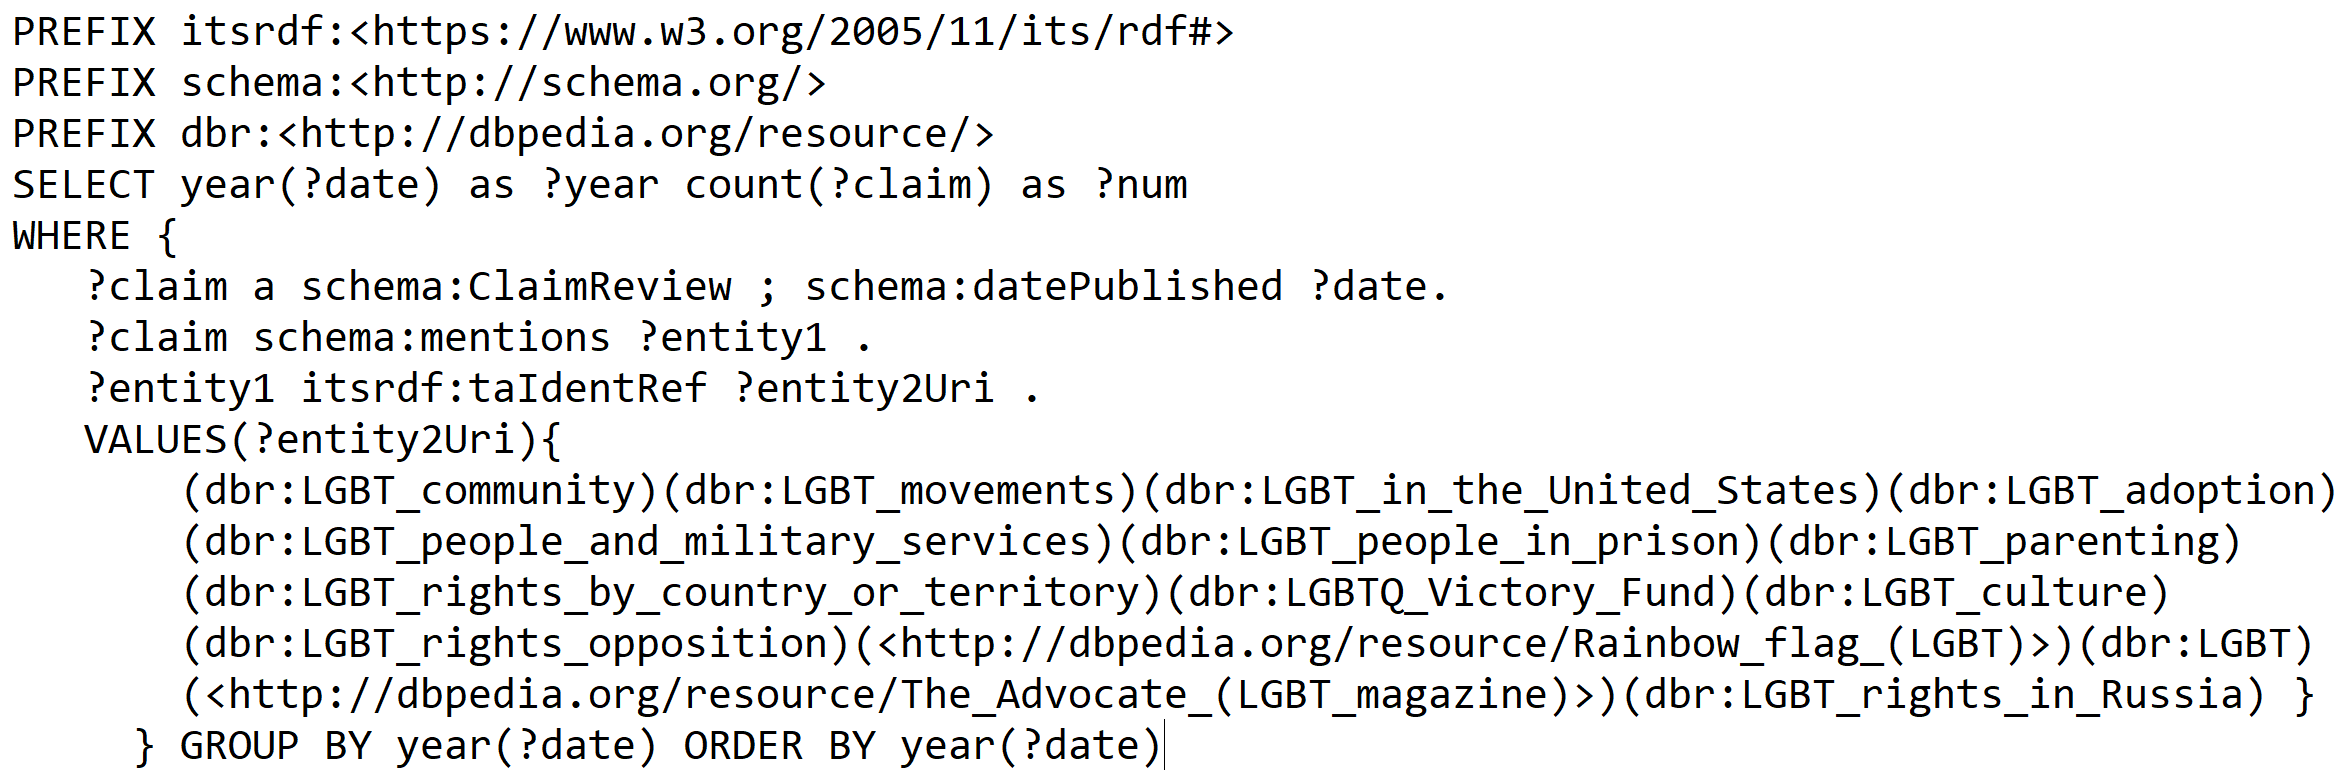
\includegraphics[width=0.70\linewidth]{test2.PNG} & 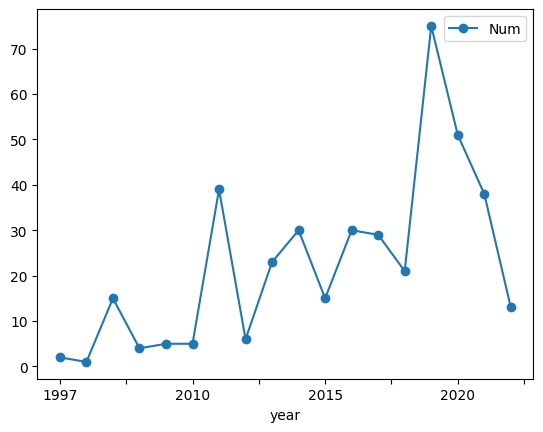
\includegraphics[width=0.25\linewidth]{lgbt.png} \\
         (a) &  (b)
    \end{tabular}
    \caption{(a) SPARQL query to fetch all claims regarding the LGBT community year-wise. (b)  Spread of LGBTQ claims from 1996-2022.}
    \vspace{-4mm}
    \label{fig:lgtb}
\end{figure}

\vspace{-1mm}
\subsection{ClaimsKG and Historical Events}
\vspace{-2mm}

The query in Figure~\ref{fig:lgtb}(a) is an example of fetching trends or important events in history. The query fetches all claims regarding the LGBT community and their corresponding year. The result of this query shows a sudden spike in the year 2018 from 2017 with a number of claims that rises from \textbf{21} to \textbf{75} (see Figure~\ref{fig:lgtb}(b)). This spike can be attributed to the event of legalizing same-sex weddings by the Australian Parliament in Dec 2017, resulting in a sudden rise in claims regarding this topic. %We have also tried other
One could look for interesting entities like ``Black lives matter", ``Global Warming"  and the ``Great Recession" which would fetch us claims regarding these topics. These queries could be particularly useful for social scientists, who are interested in studying specific phenomena at specific points in time and can find out which information (both true and false) was spreading online.
\vspace{-4mm}


\subsection{ClaimsKG and US Presidents}
%In our next example, we would like to show the use of 
\vspace{-2mm}
This example demonstrates the interesting ability of ClaimsKG to fetch information from external databases with the help of SPARQL queries. For example, the query in Figure \ref{Table6} fetches false claims regarding all Presidents of the United States who belonged to the Democratic Party. As the reader can see, the information about which president belonged to the Democratic Party is given by DBpedia and used to explore ClaimsKG. The query outputs the claim text, the review URL, the name of the President as a DBpedia resource and the claim's rating. The results display claims such as ``Barack Obama began his presidency \lq{}with an apology tour\rq{}." or  ``Joe Biden calls Pennsylvania voters who don’t support him \lq{}chumps\rq{}." which were rated as false by the fact-checkers published in the fact-checking website \textit{PolitiFact}.
\vspace{-4mm}
\begin{figure}[t]
\centering
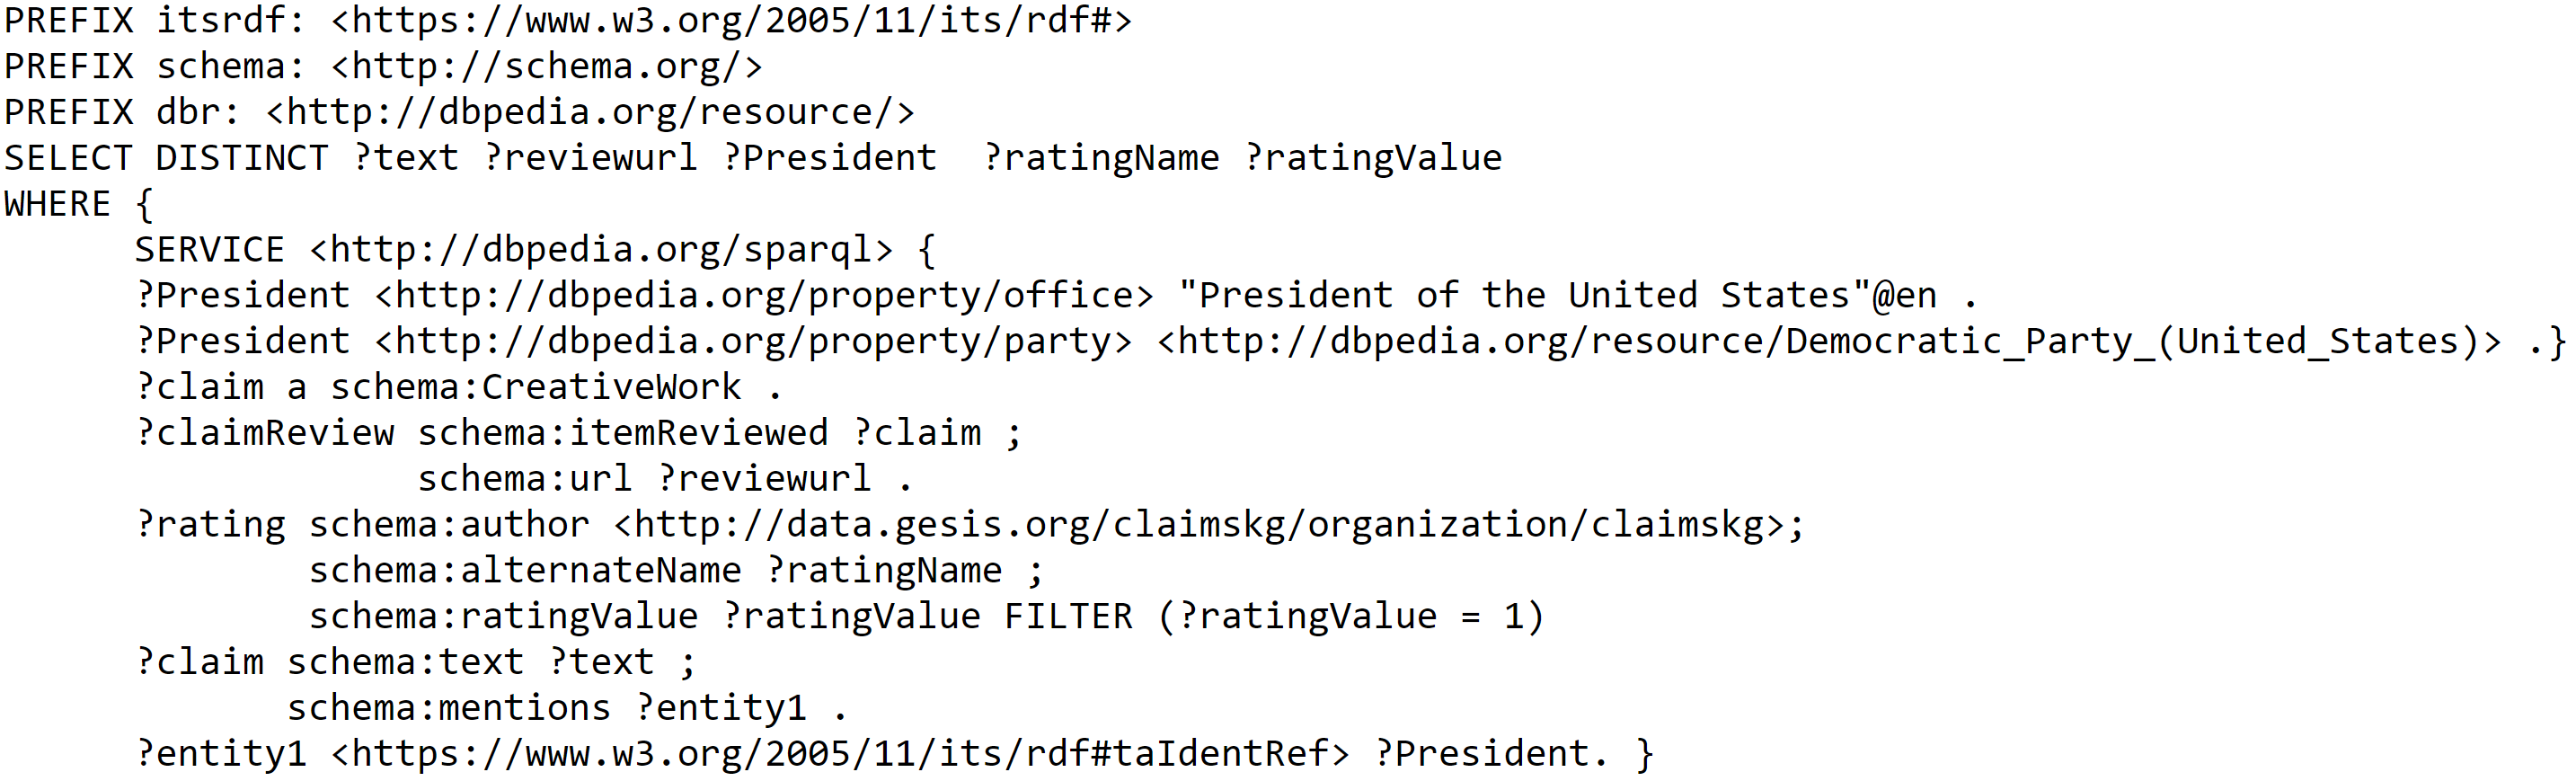
\includegraphics[width=0.7\linewidth]{table6.PNG}
\caption{SPARQL query to fetch all false claims regarding US Presidents of the democratic party}
\label{Table6}
\vspace{-4mm}
\end{figure}

\subsection{ClaimsKG and Diseases}
\vspace{-2mm}
In recent years, the spread of diseases and the number of claims regarding them have been on the rise. We tried to have a closer look at this topic. Figure \ref{fig:disease}(a) fetches claims that contain mentions of any disease in ClaimsKG.  The query outputs 806 %rows 
results along with the source review URL and the disease entity that was mentioned. Disease entities were retrieved from DBpedia. From the results, we filter out the top 5 diseases that were mentioned in these claims which show that \textit{Cancer} was the highest (Table \ref{disease_table}). Apart from the diseases mentioned in this table, there were also other diseases like Plague, Strabismus Palliative care, and others that were sparsely mentioned in the Knowledge Graph. After analysis of the veracity labels, we plot a graph of the entities and their truth values in Figure \ref{fig:disease}(b).
The plot shows that \textit{Cancer} is the most discussed and mentioned disease, and almost 47\% of the claims made about cancer are false. These included claims like ``Drinking hot coconut water kills cancer cells" or ``An association of pediatricians ``admitted” that HPV vaccine Gardasil causes ovarian ``failure” or cancer." There are very few true claims, only 0.06\% of the total which included claims like ``Four in ten cancer patients lose their life savings after starting treatment." which is highly alarming. There are mentions of other diseases like influenza, infection, diabetes, and mental disorder that are predominantly present in the Knowledge Graph. On a general inspection, it is observable that the number of false claims is always more than claims labeled as \textit{TRUE} or \textit{MIXTURE} for any kind of disease. There is also a considerable percentage of claims that are rated as \textit{OTHER} which did not have any clear rating value associated with them. For example, the claim ``Asparagus has miraculous cancer-fighting properties." published in Snopes has a rating of ``Unproven" which is clearly neither true nor false. Likewise, \textit{OTHER} claims included claims with original ratings such as ``research in progress", ``outdated", etc, and sometimes no rating attached to the claim.
\vspace{-4mm}

\begin{figure}
   \begin{tabular}{cc}
         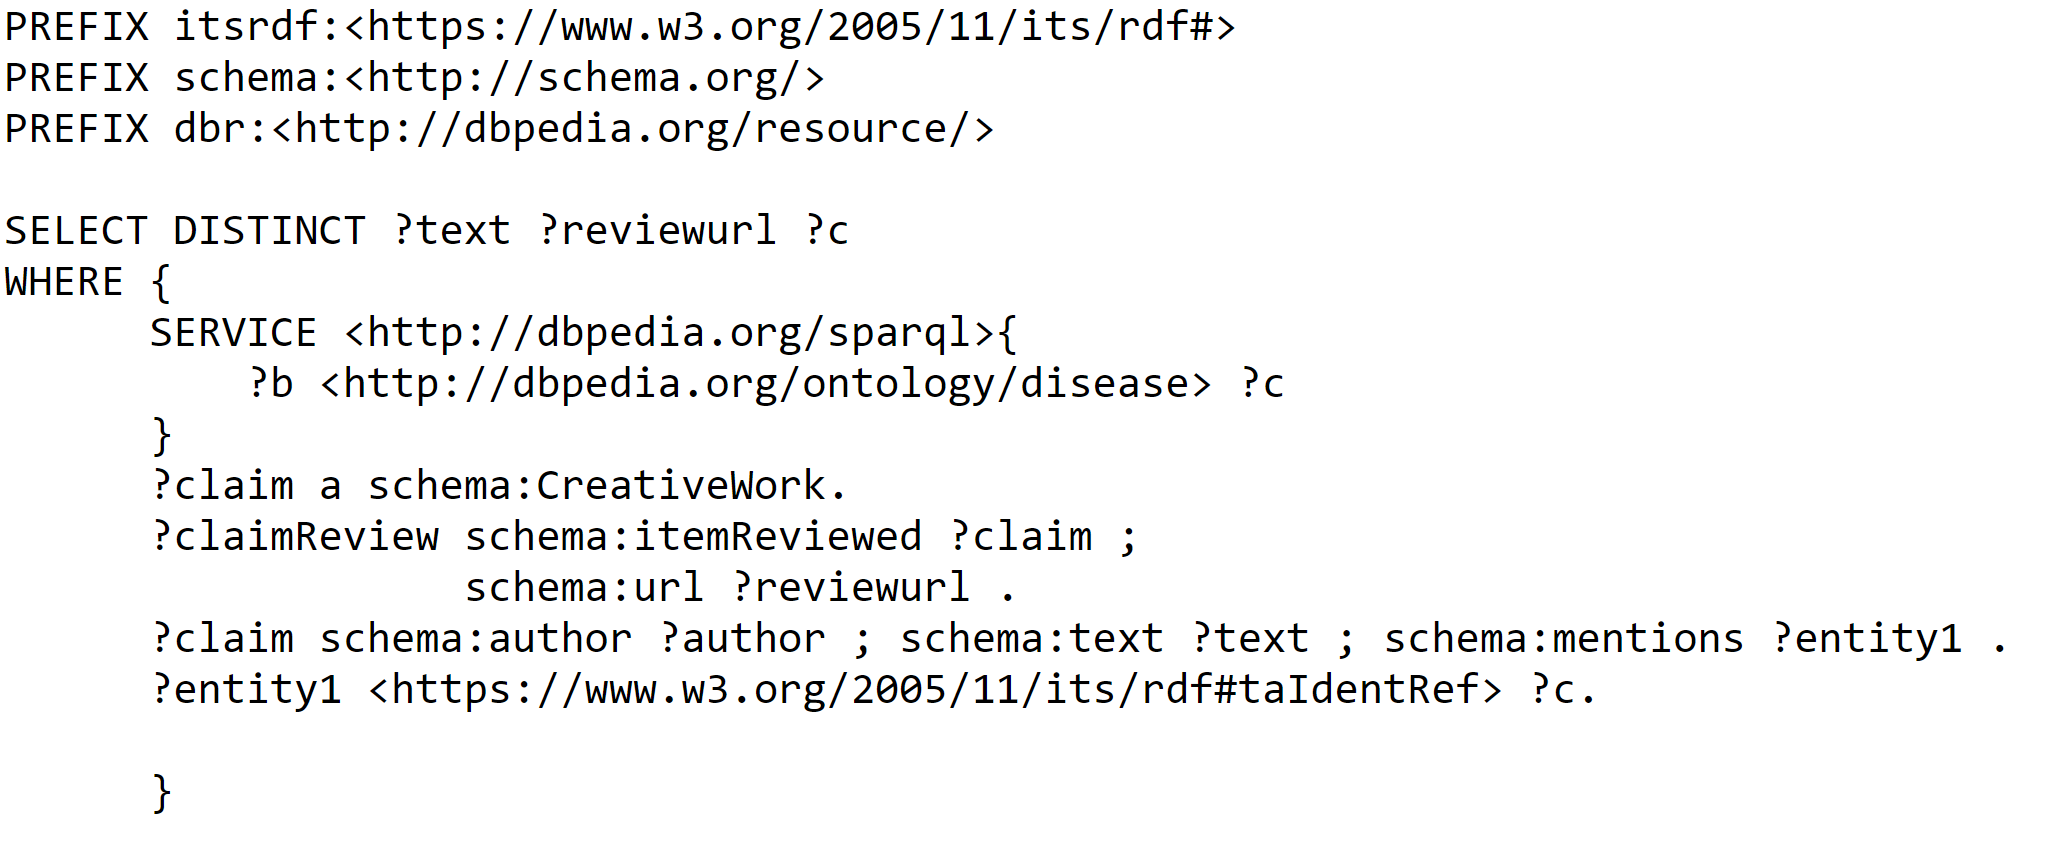
\includegraphics[width=0.65\linewidth]{table7.PNG} &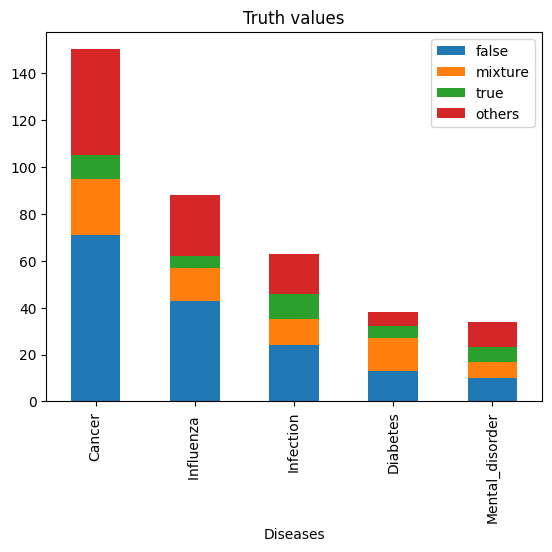
\includegraphics[width=0.30\linewidth]{diseases.png}  \\
         (a) & (b) 
   \end{tabular}
   \caption{(a) SPARQL query to fetch all claims regarding diseases mentioned in ClaimsKG. (b) Mention of disease entities and their veracity labels. }\vspace{-4mm}
\label{fig:disease}
\vspace{-4mm}
\end{figure}
\begin{table}[ht]
\scriptsize
\caption{  Top 5 disease entities that are mentioned in ClaimsKG. } \label{disease_table}
\centering
\begin{tabular}{|l|c|}

\hline
\textbf{Diseases}                            & \textbf{Counts} \\ \hline
\url{http://dbpedia.org/resource/Cancer }          & 150             \\ \hline
\url{http://dbpedia.org/resource/Influenza}        & 88              \\ \hline
\url{http://dbpedia.org/resource/Infection }       & 63              \\ \hline
\url{http://dbpedia.org/resource/Diabetes }        & 38              \\ \hline
\url{http://dbpedia.org/resource/Mental\_disorder} & 34              \\ \hline

\end{tabular}
\vspace{-4mm}
\end{table}
\vspace{-2mm}
\section{Conclusion and Future Work}
\vspace{-2mm}
We present the latest release of ClaimsKG, a knowledge graph of fact-checked claims which enables structured queries about their related metadata. We describe the pipeline changes made in this version and provide detailed statistics of the data. We also demonstrate use cases to show how 
ClaimsKG can be used for data analysis for various social-science-related research questions. %Although ClaimsKG captures a wide spectrum of important events and trends, some of the events are yet to be considered. 
We observe that the NERD tool fails to recognize some entities. This gives us the scope for further improvements. In the future, we aim to enhance the entity annotation capabilities with more focus on the social science domain.
We plan to include more sources with diverse languages and perform multilingual entity linking and disambiguation for enhancing the quality of ClaimsKG. We also intend to analyze how the same or similar claims are covered across different sources and the degree of agreement between the fact-checking websites. ClaimsKG will foster new discussions about topics related to specific domains and support users in the exploration of online truthfulness about specific facts. 
\vspace{-6mm}
\bibliography{sample-ceur}




\end{document}

%%
%% End of file
